%
%% 2019 07 04 Ph. G. Freimann
%%

\section{Lineare Gleichungen I}\index{Gleichungen!lineare}\index{lineare Gleichung}\label{gleichungen_lineare}
\sectuntertitel{... weil keine zwei Dinge gleicher sein
  können.\footnote{\textit{Robert Recorde} (1557; \textit{Der
      Wetzstein des Wissens}) über das
    Gleichheitszeichen\index{Gleichheitszeichen} als zwei Parallele:
    «... weil keine zwei Dinge gleicher sein können.»}}

\theorieTALS{81}{2.2}
\theorieGESO{115}{8}
%%%%%%%%%%%%%%%%%%%%%%%%%%%%%%%%%%%%%%%%%%%%%%%%%%%%%%%%%%%%%%%%%%%%%%%%%%%%%%%%%
\subsection*{Lernziele}

\begin{itemize}
\item Lineare Gleichungen
\item Äquivalenzumformung / Lösungsmenge
\item Grundform (GF) linearer Gleichungen
\item Textaufgaben, die zu Gleichungen\index{Textgleichungen}\TALS{
  (ev. mit Parametern)} führen.
\TALS{\item Einsatz des Taschenrechners}
\end{itemize}

\TRAINER{\GESO{Bem. «Lineare Gleichungen ohne Parameter»}}
\noTRAINER{\vspace{10mm}}

\begin{definition}{Lineare Gleichung}{definition_lineare_gleichung}
  Eine \textbf{lineare Gleichung} ist eine Gleichung, bei der die
  gesuchte Variable in der ersten Potenz ($x^1$) vorkommt.\\
  Grundform (GF)\index{Grundform!lineare Gleichung} oder Normalform\index{Normalform!lineare Gleichung}:\\
  $$ax+b=0$$
  \end{definition}

\begin{beispiel}{Grundform}{beispiel_lineare_gleichung_grundform}
  Bringen Sie die folgende lineare Gleichung auf die Grundform:
  $$2x-7+3x = 5x-6-\frac{x}{2}$$
  \TRAINER{Grundform: $\frac{1}{2}x - 1 = 0$}
  \noTRAINER{$$.......................................$$}
  \end{beispiel}


\TALS{%%
%% 2020 graphische Interpretation linearer Gleichungen (TALS nSpire)
%%


\newpage
\subsection{Graphische Interpretation}
Graphische Interpretation der Grundform:

In der Form
$$ax+b=0$$
ist $a$ die Steigung\footnote{Steigung: Eine Einheit nach rechts: Um wie viele Einheiten steigt die Gerade an?} der Geraden und $b$ der Abschnitt\index{Achsenabschnitt} auf der $y$-Achse\footnote{$y$-Achsenabschnitt: Wo schneidet die Gerade die $y$-Achse.}:

\bbwCenterGraphic{6cm}{allg/gleichungen/img/LineareGleichungsfunktion.png}
%  \begin{center}
%   \raisebox{-1cm}{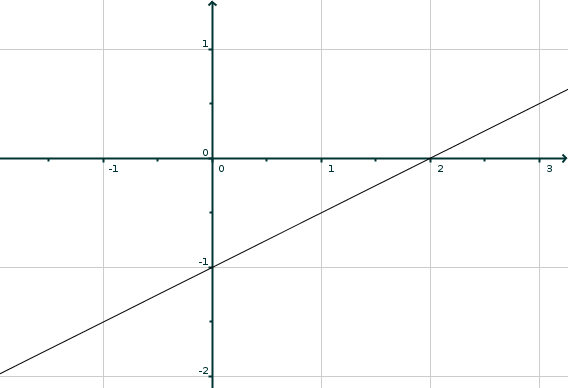
\includegraphics[width=6cm]{img/LineareGleichungsfunktion.png}}
%  \end{center}

  \paragraph{Charakteristische Punkte}
  Die charakteristischen Punkte (spezielle Punkte) der linearen
  Funktion in Grundform sind

  \begin{itemize}
  \item $b$ = $y$-Achsenabschnitt: Wo schneidet die Gerade die $y$-Achse?
  \item $a$ = Steigung der Geraden pro eine Einheit nach rechts (in $x$-Richtung)
  \item $\frac{-b}{a}$ = Lösung der Gleichung $ax+b=0$. Dies ist der $x$-Achsenabschnitt.
  \end{itemize}

}
  
  \subsection{Grundmenge, Definitionsmenge}\index{Grundmenge}\index{Definitionsmenge}
  Die Menge aller Zahlen, welche für die Lösung in Frage kommen,
  nennen wir die Grundmenge oder Definitionsmenge. Diese ist üblicherweise $\mathbb{R}$, die
  Menge der reellen Zahlen und wir schreiben:
  $$\mathbb{G}=\mathbb{R}$$
  Teilweise sind als Lösungen auch nur positive ($\mathbb{G}=\mathbb{R}^+$) oder
  beispielsweise nur ganze Zahlen ($\mathbb{G}=\mathbb{Z}$)
  zugelassen.
  Insbesondere ist die Menge der Lösungen jedoch eingeschränkt durch
  die Terme, welche die Gleichung definieren. So besteht die folgende
  Gleichung aus zwei Termen ($T1=\frac{4}{x-2}$ und $T2=\frac{\sqrt{x}}{x-3}$) mit den unten angegebenen
  Einschränkungen:
  $$\frac{4}{x-2}=\frac{\sqrt{x}}{x-3}$$
  Die Definitionsmengen von $T1$ und $T2$ schränken automatisch die
  Grundmenge der Gleichung ein. In obigem Beispiel gilt:
  
  $$\mathbb{D}_1=\mathbb{D}(T1)=\LoesungsRaum{\mathbb{R}\backslash\{2\}}$$

  $$\mathbb{D}_2=\mathbb{D}(T2)=\LoesungsRaum{\mathbb{R}^+_0\backslash\{3\}}$$

  $$\mathbb{D}=\mathbb{D}_1\cap\mathbb{D}_2=\LoesungsRaumLang{\mathbb{R}^{+}_{0}\backslash\{2;3\}}$$

  
  \subsection{Lösungsmenge}\index{Lösungsmenge}
  Die Zahlmenge, der gefundenen Lösungen einer Gleichung, nennen wir
  die Lösungsmenge und beschriften diese $\mathbb{L}$. Falls die gefundene
  Variable $x$ \zB{} den Wert $4$ hat, dann schreiben wir:
  $$\mathbb{L}_x=\{4\}$$
  Eine Gleichung ohne Lösung hat die leere Menge als Lösungsmenge und
  wir schreiben:
  $$\mathbb{L}_x=\{\}$$
  Falls alle Zahlen $x$ die Gleichung lösen, so schreiben wir:
  $$\mathbb{L}_x=\mathbb{R}$$

  
\newpage
\subsection{Äquivalenzumformungen}\index{Äquivalenzumformungen}
Äqui... = Gleich...; ...valenz = ...wertig

\TALS{S. \cite{frommenwiler17alg} Seite 79 (Äquivalenz von Aussageformen)}
\TALS{S. \cite{frommenwiler17alg} Seite 80 (Liste der Äquivalenzumformungen)}
\GESO{S. \cite{marthaler17} Seite 111 (Liste der Äquivalenzumformungen)}
\begin{itemize}
	\item Termumformungen (unabhängig links und rechts des Gleichheitszeichens, sofern der Definitionsbereich des Terms nicht verändert wird.)
	\item $\pm    c\ (c \in \mathbb{R})$
	\item $\cdot\ c\ (c \in \mathbb{R}\backslash 0)$
	\item $:      c\ (c \in \mathbb{R}\backslash 0)$
\TALS{\item $+ cx^n\ (c \in \mathbb{R}, n \in \mathbb{N}, x$ ist die Unbekannte$)$}
\end{itemize}
\newpage

\subsubsection{Finde Äquivalenzumformungen}
Der folgende Lösungsweg ist definitiv falsch. Irgendwo ist eine Umformung vorgenommen worden, die nicht gültig ist.
Schreiben Sie bei jeder Umformung hin, um welche der oben angegebenen gültigen Äquivalenzumformung es sich handelt. Finden Sie den Fehler:

Im folgenden seien $\pi$ und $a$ als die Kreiszahl $3.14159...$ definiert. Es gilt also $\pi = a$.
\begin{tabular}{lrclp{7cm}}
                  & $a$              &$=$& $\pi$               & nach Voraussetzung       \\
$\Longrightarrow$ & $a\cdot a$       &$=$& $a\cdot\pi$         & wegen .........................     \\ 
$\Longrightarrow$ & $a^2$            &$=$& $a\pi$              & ................................... \\ 
$\Longrightarrow$ & $a^2 + a^2$      &$=$& $a\pi + a^2$         & ................................... \\
$\Longrightarrow$ & $2a^2$           &$=$& $a\pi + a^2$         & ................................... \\ 
$\Longrightarrow$ & $2a^2-2a\pi$     &$=$& $a\pi + a^2 -2a\pi$  & ................................... \\ 
$\Longrightarrow$ & $2a^2-2a\pi$     &$=$& $\,\,\,\,\,\,\,\,\,\,\,\,\,\,  a^2 -a\pi$  & ................................... \\ 
$\Longrightarrow$ & $2a^2-2a\pi$     &$=$& $a\cdot(a-\pi)$     & ................................... \\ 
$\Longrightarrow$ & $2a\cdot(a-\pi)$ &$=$& $a\cdot(a-\pi)$     & ................................... \\ 
$\Longrightarrow$ & $\frac{2a\cdot(a-\pi)}{a-\pi}$ &$=$& $\frac{a\cdot(a-\pi)}{a-\pi}$     & \noTRAINER{...................................} \TRAINER{hier wurde durch 0 dividiert, denn $a=\pi$!}\\ 
$\Longrightarrow$ & $2a$             &$=$& $\frac{a\cdot(a-\pi)}{a-\pi}$     & \noTRAINER{...................................}\TRAINER{Definitionsbereich durch Termumformung links verändert} \\ 
$\Longrightarrow$ & $2a$             &$=$& $a$                 & \noTRAINER{...................................}\TRAINER{Definitionsbereich durch Termumformung rechts verändert} \\ 
$\Longrightarrow$ & $2$              &$=$& $1$                 & ........................ \\ 
\end{tabular}
\newpage

\TALS{%%
%% 2019 11 14 Ph. G. Freimann
%%

\subsection{Gleichungen mit CAS lösen}\index{CAS@Computer Algebra System}\index{Computer Algebra System@CAS}
Damit weniger Fehler geschehen, aber auch, um schneller an Resultate zu gelangen werden in der Praxis Gleichungen fast ausschließlich mit einem Computer-Algebra-System (CAS) gelöst.
Wir wählen eine einfache Gleichung, damit wir a) nicht viel tippen müssen und b) das Resultat auch sofort überprüfen können. Gegeben ist also die folgende Gleichung:

$$3x+1=2x$$

Typischerweise bieten sich die folgenden drei Lösungswege an\footnote{Die drei Verfahren wurden mit dem Rechner ``TI-nspire II-CX CAS'' getestet.}:
\begin{itemize}
\item solve($3x+1=2x$, $x$)
\item $gl1 := 3x+1=2x$\\
  solve($gl1$, $x$)
  
\item $term1 := 3x+1$\\
  $term2 := 2x$\\
  solve($term1=term2$, $x$)\\
  Diese letzte Variante hat den Vorteil, dass wir die Terme leicht als Funktionen in $x$ auffassen können und diese im Graph-Modus sofort anzeigen können:
  \begin{enumerate}
    \item Neue «Page» (1.2) erstellen (+page) als Graph. 
    \item Tippe $f1(x)=term1$
    \item Tippe \fbox{CTRL} \fbox{G} (oder mehrmals die \fbox{TAB}-Taste), um die Eingabezeile wieder zu aktivieren.
      \item $f2(x)=term2$
  \end{enumerate}

\bbwCenterGraphic{6cm}{tals/gl1/img/nspire_zwei_gleichungen.png}
%  \begin{center}
%   \raisebox{-1cm}{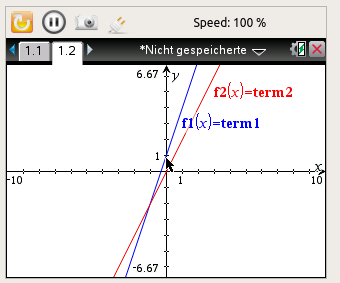
\includegraphics[width=6cm]{img/nspire_zwei_gleichungen.png}}
%  \end{center}
  Der Schnittpunkt der beiden Geraden zeigt die Variable $x$ (hier $-1$) und den Wert der beiden Terme (links bzw. rechts) des Gleichheitszeichens als Variable $y$ (hier $-2$) an.

\end{itemize}
}

\subsubsection{Spezielle lineare Gleichungen}
\textbf{Typ A}\\

$$1+4x+2 = 5x - (x-3)$$
\TNT{2.8}{$$\mathbb{L}_x = \mathbb{R}$$}

\textbf{Typ B}\\

$$3x+8 = 5x-(2x-6)$$
\TNT{2.8}{$$\mathbb{L}_x = \{\}$$}

\textbf{Grundform}\index{Grundform!lineare Gleichung}\\

\begin{beispiel}{Lineare Gleichung}{beispiel_lineare_gleichung_3x7}
  Die Gleichung $3x=-7$ ist äquivalent zur Grundform $3x+7=0$ und somit ist die Lösungsmenge $\mathbb{L}_x=\left\{ \frac{-7}{3}  \right\}$
  \end{beispiel}

\begin{beispiel}{Lineare Gleichung}{beispiel_lineare_gleichung_5x8}
  Die Gleichung $-5x=8$ ist äquivalent zur Grundform $-5x-8=0$ und somit ist die Lösungsmenge $\mathbb{L}_x=\left\{ \frac{-8}{5}  \right\}$
\end{beispiel}

Die Lösungsmenge $\mathbb{L}_x$ zur allgemeinen Grundform $ax+b=0$ lautet somit $\mathbb{L}_x=\left\{ \frac{-b}{a} \right\}$.

\begin{itemize}
  \item Im Spezialfall \textbf{Typ A} gilt $a=0$ und $b=0$. Hier kann ich für $x$ alles einsetzen und somit gilt $\mathbb{L}_x=\mathbb{R}$.
  \item Im Spezialfall \textbf{Typ B} gilt $a=0$ und $b\ne 0$. Hier wird die Gleichung falsch, egal, was ich für $x$ einsetze; somit ist $\mathbb{L}_x=\{\}$.
\end{itemize}
\newpage

\subsection*{Aufgaben}
\TALSAadB{81}{223-226}
\GESOAadB{127ff}{
  2. a) f)
  3. a) h)
  6. a) d) e) f)
}
\newpage
